\subsection{Funktionen und Oberflächen}
    \label{section:solutionDetailsWebAppFunctions}
    Die Webanwendung soll Nutzern eine größere und zugleich detailliertere
    Übersicht über Klassifikationen verschaffen,
    als dies mit Webannotationen möglich ist.
    Ihre Informationen bezieht sie dafür von der
    {\classificationStorageAPI}.
    Die erste Oberfläche der Webanwendung ist ein Dashboard
    und ist in Abbildung \ref{image:webAppDashboard} zu sehen.

    \begin{figure}[htb]
        \centering
        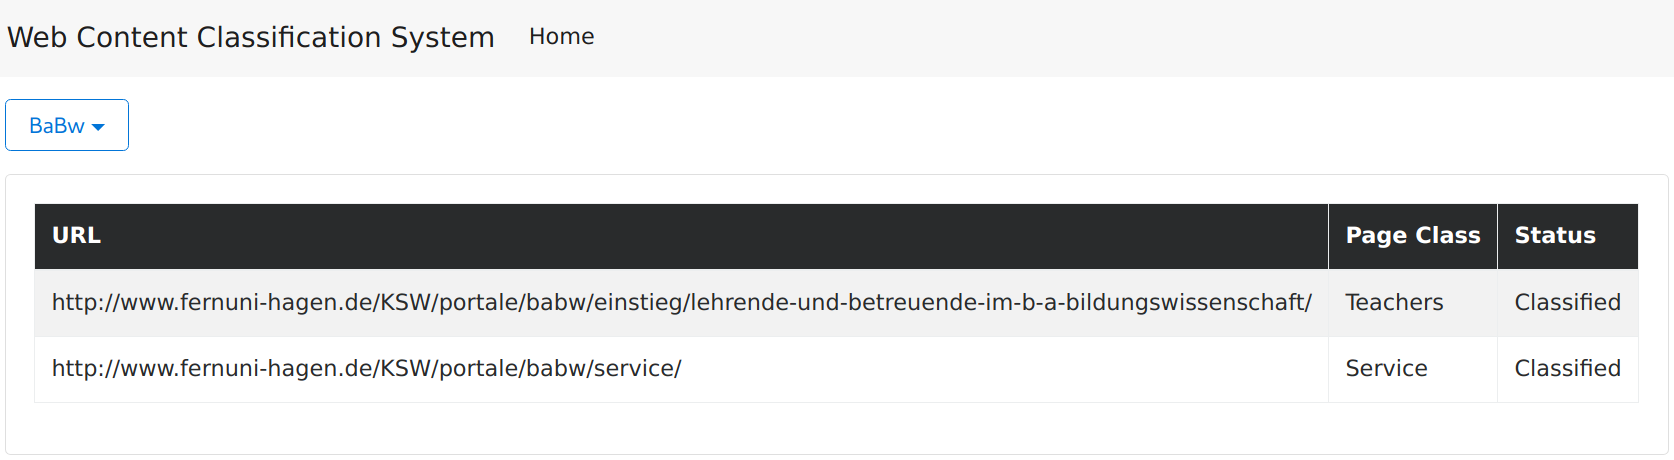
\includegraphics[width=\textwidth]{../resources/web-app/dashboard.png}
        \caption{Übersicht aller klassifizierter Webseiten in der Webanwendung}
        \label{image:webAppDashboard}
    \end{figure}

    Diese Übersichtseite enthält oben links eine Auswahlliste, die alle bekannten Sites enthält.
    Bei Auswahl einer Site wird die darunter liegende Tabelle aktualisiert.
    Diese enthält Informationen zu allen klassifizierten Webseiten der ausgewählten Site.
    Das umfasst ihre \glspl{url}, ihre Klassen und ihre Status.
    Durch einen Klick auf die Zeile einer Seite,
    gelangt man zur ihrer Detailseite,
    die in Abbildung \ref{image:webAppDetailPage} zu sehen ist.

    \begin{figure}[htb]
        \centering
        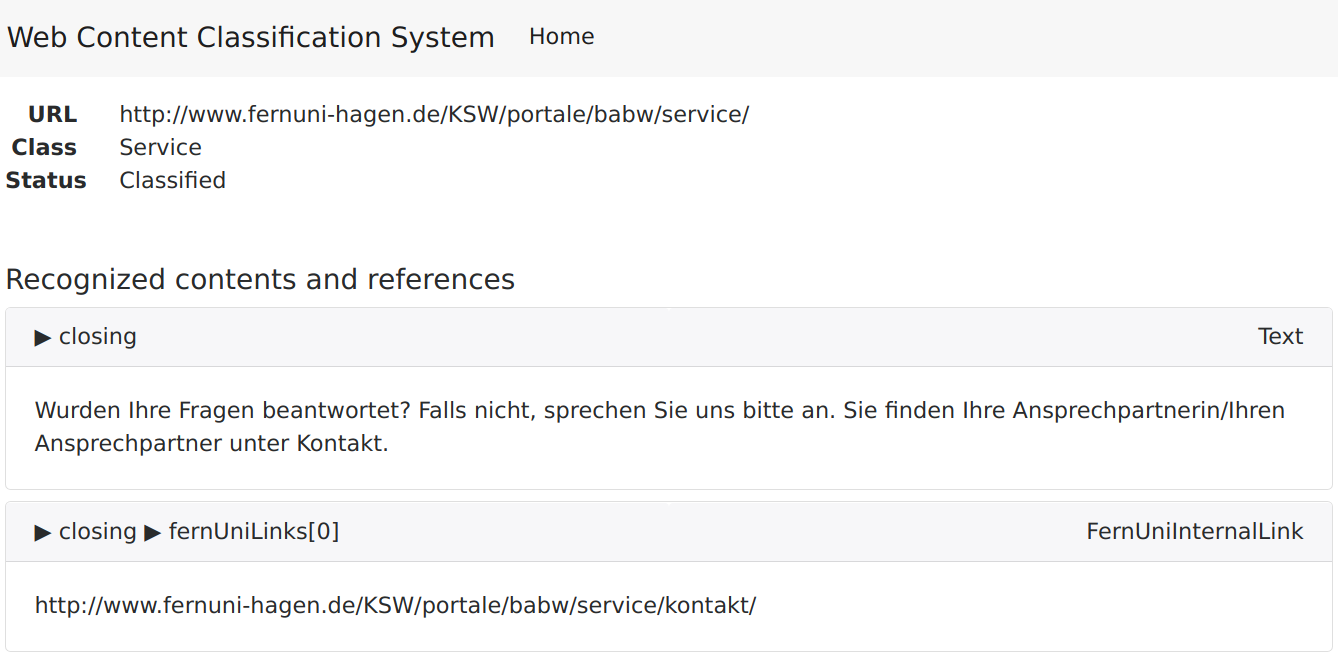
\includegraphics[width=0.8\textwidth]{../resources/web-app/detail-page.png}
        \caption{Detailseite einer klassifizierten Webseite in der Webanwendung}
        \label{image:webAppDetailPage}
    \end{figure}

    Im Kopf dieser Oberfläche sind nochmals die Informationen
    des Dashboards über die aktuelle Klassifikation aufgeführt.
    Darunter befindet sich für jedes Feature ein Abschnitt,
    der verschiedene Informationen zum jeweiligen Feature enthält.
    Oben links steht der Pfad,
    der in der Klassifikation zum Feature führt.
    Ob es sich um ein {\collectionFeature} handelt,
    kann ebenfalls aus diesem Pfad abgelesen werden.
    Der letzte Teil enthält in diesem Fall den Index des Elementes im Feature.
    Die Klasse des Features ist oben rechts zu sehen.
    Darunter befindet sich der textuelle Inhalt oder das Referenzziel
    des Features.
    Die Detailseite verzichtet bewusst darauf, auch die eindeutigen Selektoren der Features aufzuführen,
    da sie für die Prüfung der Klassifikation weniger wichtig sind,
    als die korrekte Strukturierung der Inhalte und Referenzen.
